% @Author: AnthonyKenny98
% @Date:   2020-04-08 11:48:44
% @Last Modified by:   AnthonyKenny98
% @Last Modified time: 2020-04-08 11:54:02
\begin{figure}
\begin{centering}
\begin{tabular}{c c}

    \begin{subfigure}{0.4\linewidth}
    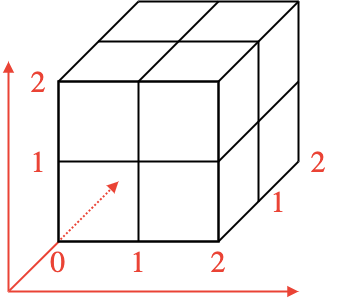
\includegraphics[width=\linewidth]{chapters/chapter3/img/honeybee_epsilon_grids_a.png}
    \caption{For $\epsilon=2$, an output collision-bit sequence of length 8 is required.}
    \end{subfigure} & 

    \begin{subfigure}{0.4\linewidth}
    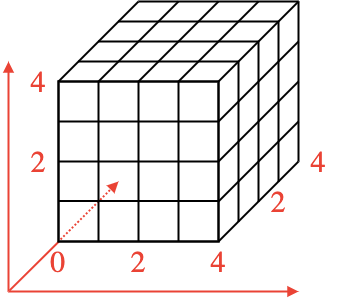
\includegraphics[width=\linewidth]{chapters/chapter3/img/honeybee_epsilon_grids_b.png}
    \caption{For $\epsilon=4$, an output collision-bit sequence of length 64 is required.}
    \end{subfigure} \\    

\end{tabular}
\mycaption{The Impact of $\epsilon$ on the Length of the Bit-Collision Sequence}{}
\label{fig:honeybee_epsilon_grids}
\end{centering}
\end{figure}